\documentclass[tikz]{standalone}
\usetikzlibrary{calc}
\usepackage{pgfplots}
\usepgfplotslibrary{polar}
\pgfplotsset{compat=1.13}

\begin{document}

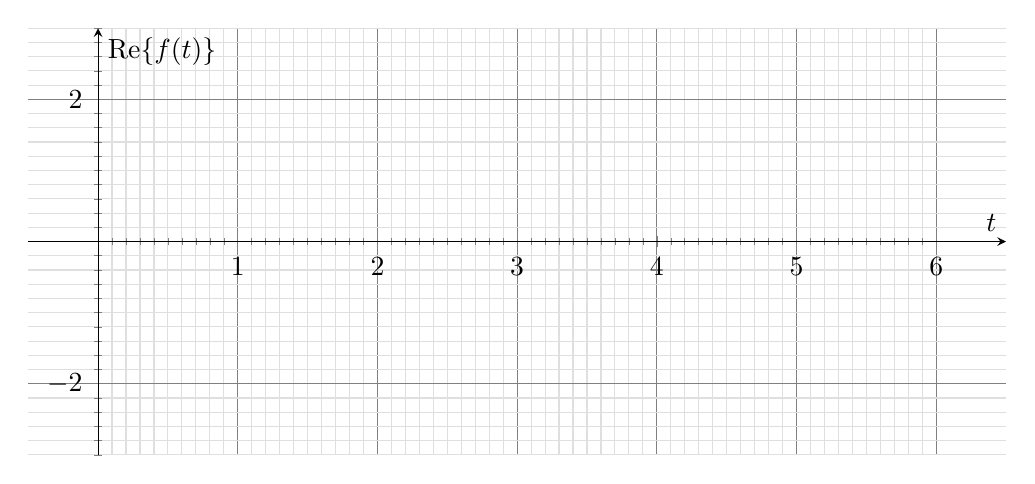
\begin{tikzpicture}
\begin{axis}[
  width=14cm,
  height=7cm,
  xlabel={$t$},
  ylabel={$\mathrm{Re} \{f(t)\}$},
  axis lines=middle,
  xmin=-.5,
  xmax=6.5,
  ymin = -3, ymax = 3,
  xtick = {0, 1,2,3,4,5,6},
  grid = both,
  minor tick num=9,
  minor grid style={gray!25},
  major grid style={black!50},
]

%\addplot+[white, ycomb, domain=-2:10, samples=13,variable=k] { (k==0)}; 

\end{axis}
\end{tikzpicture}
\end{document}
